\documentclass[authoryear, 12pt,5p, times]{elsarticle}
\usepackage[hypcap]{caption}
\usepackage{float}
\usepackage{amsmath}
\usepackage[hidelinks]{hyperref} 
 \usepackage{gensymb}
\usepackage{subcaption}
\usepackage{url}
%\renewcommand\thefootnote{\fnsymbol{\dagger}}
\usepackage[symbol*]{footmisc}
\begin{document}
%\footnote{This is a footnote}
\begin{frontmatter}
\title{Photon Counting \& the Statistics of Light}
\author{\today \\ \quad \\Jung Lin (Doris) Lee\\ dorislee@berkeley.edu\\Group partners: Jennifer Ito, Manuel Silvia\\Prof. James Graham, UGSI Heechan Yuk, Isaac Domagalski}
	\begin{abstract}
    %key objective, method, principle conclusion 
	ABSTRACT HERE
	\end{abstract}
\end{frontmatter}
\section{Introduction\label{intro}}
Spectra important chemical composition 
spectra provides composition detail to planetary bodies , stars, also the surrounding medium 
analysis
Recent development in +++++ Baryon Oscillation Spectroscopic Survey (BOSS; Dawson et al.)

is a result of each CCD pixel's different sensitivity to photon
\begin{figure}
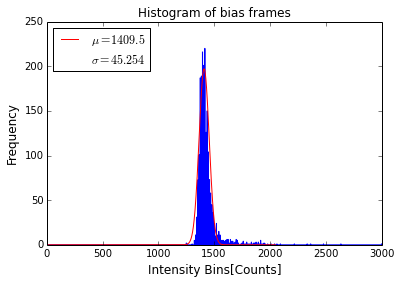
\includegraphics[width=0.5\textwidth]{figures/bias_histo}
\caption{We took a dataset of 1s integration time bias frames by placing the red cap on the spectrometer and in a black bag. A histogram of dark counts is fitted to a Gaussian. The variance of the distribution relates to the read noise and gain of the spectrometer \citep{ccd_handbook}.}
\end{figure}
\section{Experiment and }
\subsection{Spectra property and comparison for different sources}
\section{Data Reduction}
	\subsection{Automated centroid algorithm}
	find the local maxima and minima by comparing subsequent data points and testing the boolean condition of function increasing or decreasing.
	\subsection{Systematic Effects}
	 \subsection{Natural Broadening Effect}
 As seen in Fig. (LABEL HERE) the spectral lines are not perfect sharp Dirac Delta functions. This broadening is due to several physical phenomena, one reason is the natural line width caused by the measurement uncertainty inherent from quantum mechanics. Another more dominant effect is due to Doppler shift from the thermal velocity of the atoms. The distribution of the atomic thermal velocity is governed by the Boltzmann distribution. This Doppler-shifted velocity distribution propagates to our intensity measurement, which can then be rearranged into a Gaussian form. The broadening effect is chracterized by the variance of this new distribution as shown in  Eq. \ref{doppler_var},
 \begin{equation}\label{doppler_var}
\sigma_f = \sqrt{\frac{kT}{mc^2}}f_0
 \end{equation}
 where T is the temperature, m is the mass of the atom, $f_0$ is the frequency when atom is stationary, c is the speed of light and k is the Boltzman factor.
 
 \subsection{Dark Counts}
 
source of error: 
- ununiform pixels(REF dark counts)
- multiple mixed source since roomlight not closed when taking data, so slight traces of other sources in our pure data like neon...etc
 
\section{Conclusion}

Possible extension to this project may be to try conducting a basic flat-field correction to the detector. One way to do this to shine bright light uniformly on the detector to see the response of each pixel.  The exposure time needs to be short so that the CCD is not saturated. We can also try to measure maximum ranges at which CCD is sensitive and linear.
\bibliography{references}
 %\bibliographystyle{abbrvnat}
%\bibliographystyle{apalike}
%\bibliographystyle{plainnat}
%\bibliographystyle{unsrtnat}
\bibliographystyle{elsarticle-harv}
Haken, Hermann and Wolf, Hans Christolph, The Physics of Atoms and Quanta, 5th Ed., Springer-Verlag, 1996.
\end{document}
